% !TeX spellcheck = cs_CZ
\documentclass[ 12pt, a4paper]{article}
\usepackage{lmodern}
\usepackage[utf8]{inputenc}
\usepackage[czech]{babel}
\usepackage{hyperref}
\usepackage{graphicx}
\usepackage{caption}
\usepackage{indentfirst}
\usepackage{listings}
\usepackage{color}
\usepackage{amsmath}


\definecolor{dkgreen}{rgb}{0,0.6,0}
\definecolor{gray}{rgb}{0.5,0.5,0.5}
\definecolor{mauve}{rgb}{0.58,0,0.82}

\lstset{frame=tb,
	language=php,
	aboveskip=3mm,
	belowskip=3mm,
	showstringspaces=false,
	columns=flexible,
	basicstyle={\small\ttfamily},
	numbers=none,
	numberstyle=\tiny\color{gray},
	keywordstyle=\color{blue},
	commentstyle=\color{dkgreen},
	stringstyle=\color{mauve},
	breaklines=true,
	breakatwhitespace=true,
	tabsize=3
}


\begin{document}
\def\code#1{\texttt{#1}}

\pagenumbering{gobble} %bez cisel
%
%Titulni strana
\centerline{
\includegraphics[width=12cm]{logo.png}}
\vspace*{50px}
\begin{center}
	{\LARGE\bf\noindent KIV/UIR \\ Klasifikace dokumentů}\\
	\vspace*{40px}  
	
	Tomáš Ott\\
	(A17B0314P)\\
	90 hodin \\
	\vspace*{\fill}  
	\hspace*{\fill} \today \\
\end{center}
\newpage
%Obsah
\tableofcontents
\newpage

%%%%%%%%%%%%%%%%%%%%%%%%%%%%%%%%%%%%%
%%%%%%%%%%%%%%%%%%%%%%%%%%%%%%%%%%%%%
%%%%%%%%%%%%%%%%%%%%%%%%%%%%%%%%%%%%%
\pagenumbering{arabic}

\section{Zadání}
Ve zvoleném programovacím jazyce navrhněte a implementujte program, který umožní klasifikovat textové dokumenty do tříd podle jejich obsahu, např. počasí, sport, politika, apod. Při řešení budou splněny následující \\
podmínky:
\begin{itemize}
	
\item Použijte data z českého historického periodika Posel od Čerchova“, která jsou k dispozici na \url{https://drive.google.com/drive/folders/1mQbBNS43gWFRMHDYdSkQug47cuhPTsHJ?usp=sharing}. V původní podobě jsou data k dispozici na \url{http://www.portafontium.eu/periodi\\cal/posel-od-cerchova-1872?language=cs.}

\item Pro vyhodnocení přesnosti implementovaných algoritmů bude NUTNÉ vybrané dokumenty ručně označkovat. Každý student ručně anotuje 10 stran zadaného textu –
termín 31.3.2020. Za dodržení termínu obdrží student bonus 10b.

\item Přiřazení konkrétních textů jednotlivým studentům spolu s návodem na anotaci a příklady je uloženo spolu s daty na výše uvedené adrese, konkrétně:
	\begin{itemize}
	\item 0 - vzorová složka (takhle by měl výsledek vypadat)
	\item 1, 2, .. , 15, 101, 102, .. - data k anotaci
	\item přiřazení souboru studentum.xlsx - určení, jaké soubory má jaký student	anotovat. Až budete mít anotaci hotovou, doplňte sem informaci.
	\item Anotační příručka - návod, jak články anotovat.
	\item Klasifikace dokumentů - kategorie.xlsx - seznam kategorií k anotaci s příklady.
	\item sem prace20.pdf - Zadání semestrální práce
	\end{itemize}

\item implementujte alespoň tři různé algoritmy (z přednášek i vlastní) pro tvorbu příznaků reprezentující textový dokument.

\item implementujte alespoň dva různé klasifikační algoritmy (klasifikace s učitelem):
	\begin{itemize}
	\item Naivní Bayesův klasifikátor
	\item klasifikátor dle vlastní volby
	\end{itemize}

\item funkčnost programu bude následující:
– spuštění s parametry:\\
\textbf{název klasifikátoru, soubor se seznamem klasifikačních tříd, trénovací množina, testovací množina, parametrizační algoritmus, klasifikační algoritmus,název modelu}\\
program natrénuje klasifikátor na dané trénovací množině, použije zadaný parametrizační a klasifikační algoritmus, zároveň vyhodnotí úspě- šnost klasifikace a natrénovaný model uloží do souboru pro pozdější použití (např. s GUI).– spuštění s jedním parametrem:\\
\textbf{název klasifikátoru, název modelu} \\
program se spustí s jednoduchým GUI a uloženým klasifikačním modelem. Program umožní klasifikovat dokumenty napsané v GUI pomocí klávesnice (resp. překopírované ze schránky).

\item ohodnoťte kvalitu klasifikátoru na dodaných datech, použijte metriku přesnost (accuracy), kde jako správnou klasifikaci uvažujte takovou, kde se klasifikovaná třída nachází mezi anotovanými. Otestujte všechny konfigurace klasifikátorů (tedy celkem 6 výsledků).
\end{itemize}


Poznámky:
\begin{itemize}
\item pro vlastní implementaci není potřeba čekat na dokončení anotace. Pro průběžné testování můžete použít korpus současné češtiny, který je k dispozici na \url{http://ctdc.kiv.zcu.cz/} (uvažujte pouze první třídu dokumentu podle názvu, tedy např.
dokument 05857 zdr ptr eur.txt náleží do třídy zdr“ - zdravotnictví).
”
\item další informace, např. dokumentace nebo forma odevzdávání jsou k dispozici na CW pod záložkou Samostatná práce.

\end{itemize}
\newpage


%%%%%%%%%%%%%%%%%%%%%%%%%%%%%%%%%%%%%
%%%%%%%%%%%%%%%%%%%%%%%%%%%%%%%%%%%%%
%%%%%%%%%%%%%%%%%%%%%%%%%%%%%%%%%%%%%
\section{Analýza zadání}

Tato semestrální práce je zaměřena na vytvoření programu, který bude schopen pomocí trénovací množiny dat automaticky určit v jaké se předaný text nachází klasifikační třídě. Tento vstupní řetězec může patřit do několik tříd. Pro dosažení této vlastnosti je potřeba program naplnit trénovacími daty, ze kterých se naučí jak klasifikovat nové vstupní řetězce. Tato data musí obsahovat takový text, který je označkován tak, že víme do jakých klasifikačních tříd patří.

\subsection{Algoritmy pro tvorbu příznaků}
Pro dodržení jedné z potřebných vlastností klasifikace je potřeba zvolit vhodný způsob reprezentace textu. Text může být reprezentován jako vektor a nebo třeba jako slovník. V úvahu připadají algoritmy příznaků jako jsou Word2vec, N-gram nebo třeba neuronové sítě. Jelikož potřebujeme tři rozdílné příznakové metody budeme si je muset pečlivě vybrat.

Metody příznaků, které hledají nějakou souvislost v textu pravděpodobně selžou. To může být způsobené převážně nedostatečně kvalitní trénovací množinou.

Pokud si projdeme trénovací množinu souborů, tak je zřejmé, že se tam budou často vyskytovat slova, které jsou nějak znehodnocena a tudíž nemají v našem dokumentu význam. S těmito slovy je možné se vypořádat pomocí tak zvaného "stemmingu". Po této proceduře je slovo očistěno o nepotřebné přípony a případné chyby. 


\subsubsection{N-gram}
N-gram je takový způsob reprezentace textu, kde N značí počet slov, které jsou spolu spojeny do jednoho prvku. Je to tedy takový algoritmus, který počítá kolikrát se jednotlivé prvky vyskytují v dokumentu. Tento počet slov je dále rozdělen mezi dílčí klasifikační třídy.

\newpage
Nejzákladnějším reprezentantem této skupiny je "Bag of words" (1-gram) neboli pytel slov znázorněný v bloku č.\ref{lst:code1}. 
 
\begin{lstlisting}[caption={Ukázka příznakové metody "bag of words"},label={lst:code1}]
Sentences:
s1: 'Everyone need machine learning!'
s2: 'Not everyone can get that the machine learning is for everyone'

Vocabulary:
['everyone', 'need', 'machine', 'learning', 'not', 'can', 'get', 'that', 'the', 'is', 'for']
Bag of Words representation:
b1: [1 1 1 1 0 0 0 0 0 0 0]
b2: [2 0 1 1 1 1 1 1 1 1 1]
\end{lstlisting}

\subsubsection{TF-IDF}

TF-IDF je taková reprezentace, která dokáže znehodnotit slova, která jsou dokumentech často používaná. Naopak ale dokáže zvýraznit slova, která jsou danou třídy specifická.

Platí následující vztah:

\begin{equation*}
	w_{i,j} = tf_{i,j} * \log(N/df_{i}) 
\end{equation*}


kde $tf_{i,j}$ vyjadřuje četnost slova i v dokumentu j, N je počet všech klasifikačních tříd a $df_i$ je počet tříd, ve kterých se vyskytuje slovo i.


\subsection{Klasifikační algoritmy}
Existuje mnoho způsobů, jak klasifikovat textový dokument. Mezi ty nejpoužívanější patří například Naivní Bayes. Naopak složitějším způsobem, jak klasifikovat dokumenty, by bylo použití neuronových sítí. Ve všech případech jsou potřeba taková trénovací data, která jsou již zařazena do jednotlivých tříd, jež budou použity pro trénování programu. 
Naší úlohou je si vyzkoušet dvě metody klasifikátorů. V úvahu připadá klasifikace kromě zmíněného Naivní Bayese taky K-nejbližších sousedů, k-Means nebo také metody podpůrn- ých vektorů. 

\subsubsection{Naivní Bayes}

Tento jednoduchý pravděpodobnostní klasifikátor vycházející z Bayesovy věty, podle které platí následující vztah:
\begin{equation*}
P(A | B) = \frac{P(B|A)P(A)}{P(B)}
\end{equation*}

Použití tohoto klasifikátoru předpokládá, že jednotlivé evidence (příznaky) jsou podmíněně nezávisle při platnosti hypotézy H. Toto však často neplatí a proto se tento klasifikátor nazývá naivním.


\subsubsection{K-nejbližších sousedů}

K-nejbližších sousedů (neboli k-NN) je algoritmus strojového učení pro rozpoznávání vzorů.

\begin{figure}[!b]
	\centering
	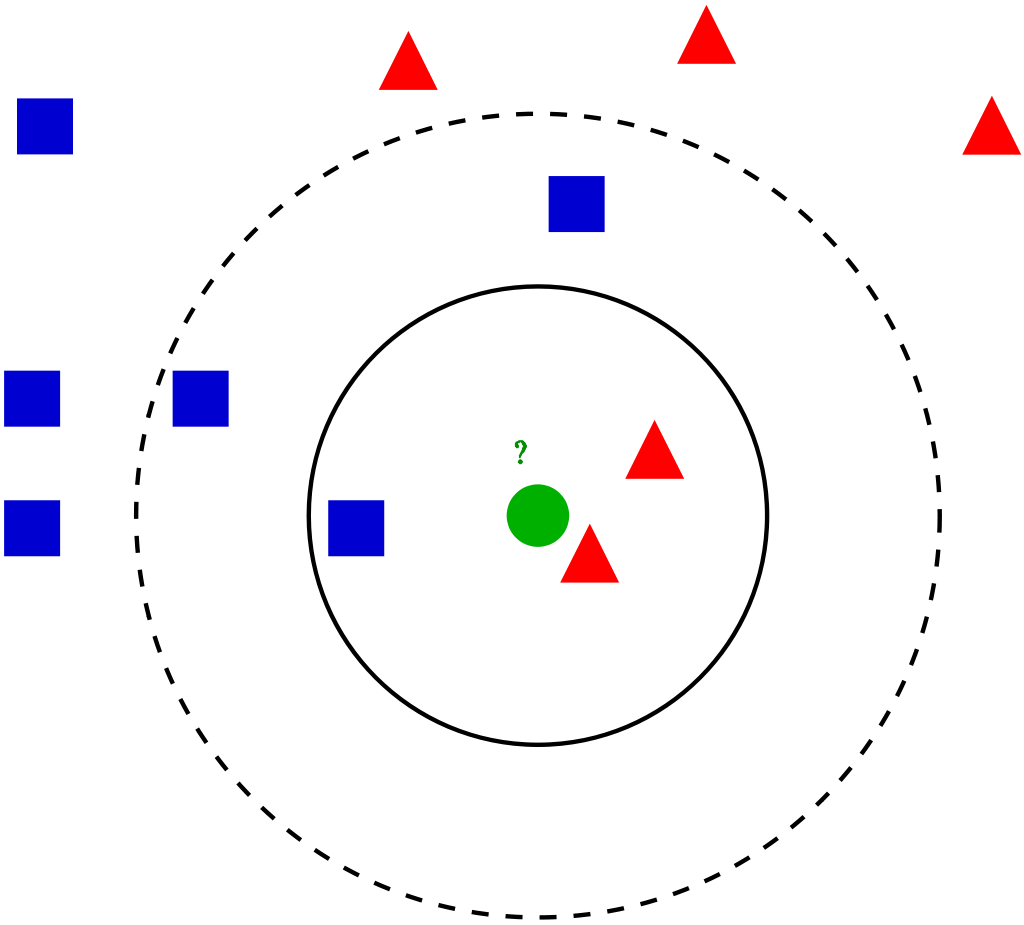
\includegraphics[width=0.7\linewidth]{knn}
	\caption{Ukázka klasifikátoru tří nejbližších sousedů (3-NN)}
	\label{fig:knn}
\end{figure}


Jde o metodu pro učení s učitelem, kdy se klasifikují prvky reprezentované více dimenzionálními vektory do dvou nebo více tříd. Ve fázi učení se předzpracuje trénovací množina tak, aby všechny příznaky měly střední hodnotu 0 a rozptyl 1 - toto umístí každý prvek trénovací množiny do některého místa v N-rozměrném prostoru. Ve fázi klasifikace umístím dotazovaný prvek do téhož prostoru a najdu k nejbližších sousedů. Objekt je pak klasifikován do té třídy, kam patří většina z těchto nejbližších sousedů.

%%%%%%%%%%%%%%%%%%%%%%%%%%%%%%%%%%%%%
%%%%%%%%%%%%%%%%%%%%%%%%%%%%%%%%%%%%%
%%%%%%%%%%%%%%%%%%%%%%%%%%%%%%%%%%%%%
\newpage
\section{Implementace}
Pro tento problém je ideální si zvolit jazyk Python. Ten totiž obsahuje v oboru strojového učení spousty knihoven, které mi pomohly jednoduše optimalizovat můj kód. Dále tento jazyk není tak verbální jako je například Java. Na časté optimalizační problémy, kdy je potřeba pracovat s vektory, slouží knihovna numpy, která má všechny své metody dobře optimalizované.

\subsection{Obsah vstupních dat}
První řádka vstupního souboru jsou třídy do kterých je text zařazen. Mezi tyto třídy patří:
\begin{itemize}
	\item ces - Cestování
	\item dop - Doprava
	\item fin - Finančnictví a obchod
	\item kri - Kriminalita
	\item kul - Kultura
	\item nab - Náboženství
	\item nes - Neštěstí a katastrofy
	\item pol - Politika
	\item pri - Příroda a počasí
	\item pru - Průmysl
	\item reg - Region
	\item rek - Reklama
	\item sko - Školství
	\item slu - Služby
	\item soc - Sociální problematika
	\item spo - Sport
	\item ved - Věda a technika
	\item voj - Vojenství
	\item zdr - Zdravotnictví
	\item zem - Zemědělství
	\item err - Error
	\item ost - Ostatní
\end{itemize}


\subsection{Naivní Bayes}

Má původní implementace tohoto klasifikátoru byla velmi neefektivní. Samotná tvorba příznaků a následná klasifikace trvala i desítky sekund. Velice mi pomohlo když jsem místo standardní konstrukce listu použil hash set. Procházení vytvořeného slovníku je nyní bleskově rychlé. Celý proces momentálně doběhne do sekundy. Jelikož jsem v jazyce Python začátečníkem, tak tahle optimalizace byla pro mě velmi složitá a zabrala spoustu času.\\ Za výsledek optimalizace jsem velmi rád.

\subsection{K-nejbližších sousedů}
Mé první pokusy o tento klasifikátor skončily neúspěchem. Pro klasickou prezentaci pomocí 1-gramu jsem dostával velice špatné výsledky. Vyřešil jsem to tak, že každý vstupní soubor jsem zařadil jako samostatný vektor. Ten byl zařazen do své skupiny a tvoří tak množinu prvků. Při klasifikování vstupního textu pak hledáme k nejbližších prvků podle Euklidovské vzdálenosti:

Třída, která je nejobsáhlejší v těchto zvolených prvcích je přiřazena pro tento vstupní text.

\subsection{Testování přesnosti}
Samotný proces ověřování přesnosti klasifikátoru je sestaven z několika procesů. Nejdříve se načtou klasifikované texty z trénovacích dat do příznakové metody. Po načtení dat následuje klasifikace jednotlivých testovacím souborů, které jsou podobné těm trénovacím. Výsledek klasifikátoru je pak porovnán se skutečností a započítán do celkové statistiky. Jakmile je tento proces dokončen je vypsána na obrazovku úspěšnost. Ta se vypočítá následovně:

\begin{equation*}
Accuracy =\frac{classified\_tags\_count}{all\_tags\_count}
\end{equation*}
\\



\begin{table}
	\begin{tabular}{||c c c c||}
		\hline
		Příznaková metoda & Klasifikátor & Potřebný čas (v sec) & Přesnost\\ 
		\hline\hline
		Bag & Naivní Bayes & 0,25 + 0,16 & 54,5\% \\ [1ex]
		\hline
		TF-IDF & Naivní Bayes & 0,33 + 0,34 & 41,57\% \\ [1ex]
		\hline
		Bigram & Naivní Bayes & 0,56 + 0,35 & 32,58\% \\ [1ex]
		\hline
		Bag & k-NN & 7,23 + 3,78 & 38,2\% \\ [1ex]
		\hline
		TF-IDF & k-NN & 7,29 + 3,78 & 40,45\% \\ [1ex]
		\hline
		Bigram & k-NN & 49,1 + 7,83 & 42,69\% \\ [1ex]
		\hline
	\end{tabular}
\caption{Kombinace všech klasifikátorů a příznakových metod}
\label{tab:acc}
\end{table}


Z tabulky je zřejmé, že implementovaný Naivní Bayes je mnohokrát rychlejší než testování pomocí klasifikátoru k-NN. To je způsobeno přetvářením jednotlivých struktur na vektory, které k-NN vyžaduje. 

Dále si můžeme všimnout, že bigram není úplně kvalitním řešením pro tento problém, protože se v trénovacích datech vyskytuje spousty nesmyslných slov, které v testovací množině nikdy nenalezneme. Při použití k-NN však dostáváme lepší výsledky, ale za cenu mnohokrát pomalejší klasifikace.


%%%%%%%%%%%%%%%%%%%%%%%%%%%%%%%%%%%%%
%%%%%%%%%%%%%%%%%%%%%%%%%%%%%%%%%%%%%
%%%%%%%%%%%%%%%%%%%%%%%%%%%%%%%%%%%%%

\newpage
\section{Uživatelská příručka}
\subsection{Nápověda}
Vypsat nápovědu pro vstupní parametry je možné pomocí příkazu:\\
"\texttt{python Main.py -h}"\\
Zde jsou vysvětleny všechny parametry, které aplikace přijímá. Mezi ně patří:
\begin{itemize}
	\item \texttt{-c <soubor\_se\_seznamem\_klasifikacnich\_trid>} soubor, který obsahuje seznam všech tříd vyskytujících se v jednotlivých dokumentech.
	\item \texttt{-train <trenovaci\_mnozina>} množina souborů, která se využije pro naplnění příznakové struktury.
	\item \texttt{-test <testovaci\_mnozina>} množina souborů, která budou využity pro ověření funkčnosti klasifikátoru.
	\item \texttt{-p <parametrizacni\_algoritmus>} parametrizační algoritmus pomocí kterého budou reprezentovány jednotlivé dokumenty. (Pouze u trénova- cího režimu) 
	\item \texttt{-k <klasifikacni\_algoritmus>} klasifikační algoritmus, který je využit pro klasifikaci dokumentů. (Pouze u trénovacího režimu)
	\item \texttt{<nazev\_modelu>} název souboru do kterého je model ukládán a v případě testovacího režimu načítán.
\end{itemize}

\subsection{Trénovací režim}
Tento režim je možné spustit zadáním následujícího příkazu:\\
"\texttt{python Main.py -c <soubor\_se\_seznamem\_klasifikacnich\_trid> 
	\\-train <trenovaci\_mnozina> -test <testovaci\_mnozina> 
	\\-p <parametrizacni\_algoritmus> -k <klasifikacni\_algoritmus> 
	\\<nazev\_modelu>}"\\

Trénovací režim neobsahuje uživatelské rozhraní a všechny jeho výstupy jsou vypisovány do terminálu. Program nejdříve naplní trénovací množinu souborů do zvolené parametrizační struktury. Poté následuje jednotlivé klasifikování testovací množiny souborů, kde po každé klasifikaci je  výsledek vypsán na obrazovku. Po dokončení druhé fáze následuje vypočtení přesnosti klasifikátoru.


\subsection{Testovací režim}
Tento režim je možné spustit zadáním následujícího příkazu:\\
"\texttt{python Main.py <nazev\_modelu>}"\\
Aplikace načte předaný model díky kterému vytvoří instance klasifikátoru a struktury příznaků. Tento model je poté využíván pro klasifikaci textu zadaného uživatelem do jednoduchého uživatelského rozhraní zobrazeno na obrázku \ref{fig:screenshot001}. 

 \begin{figure}
 	\centering
 	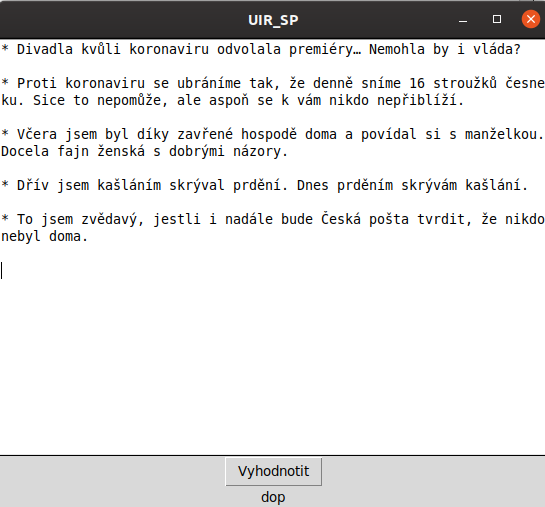
\includegraphics[width=0.7\linewidth]{screenshot001}
 	\caption{Jednoduché uživatelské rozhraní při testovacím režimu}
 	\label{fig:screenshot001}
 \end{figure}
 

%%%%%%%%%%%%%%%%%%%%%%%%%%%%%%%%%%%%%
%%%%%%%%%%%%%%%%%%%%%%%%%%%%%%%%%%%%%
%%%%%%%%%%%%%%%%%%%%%%%%%%%%%%%%%%%%%
\newpage
\section{Závěr}
Implementované metody navrací hodnoty, které bych od nich očekával. Klasifikační úspěšnost je však možné vylepšit při použití lepší trénovací množ- iny.

Mezi největší problém na který jsem při tvorbě této aplikace narazil, bylo, se zorientovat v obrovském množství materiálů dostupného na internetu. Většina pouze jednoduše popsala problém a dále odkázala na knihovnu, které ho pak za ně jednoduše vyřešila. 

Dále jsem během implementování jednotlivých algoritmů narazil v jazyce "python" na problém neefektivního zápisu polí. Samotné pole obsahují pouze ukazatele na jednotlivé prvky a to nejen pro objekty ale i pro primitivní typy. Řešení nabízí knihovna "numpy", která tento problém jazyku řeší tak, jak to funguje v každém jiném nízkoúrovňovém jazyku. 






\newpage

\end{document}